\section{Model dependence of the signal acceptance}
\label{sec:modeldependence}

The signal acceptance for T2tt events has a significant dependence on the model parameters, particularly the mixing angle of left- and right-handed stops.
Depending on the choice of mixing angle, the top quarks produced in the decay can have a polarization anywhere between
$+p_{\chi_1^0}/E_{\chi_1^0}$ and $-p_{\chi_1^0}/E_{\chi_1^0}$~\cite{0811.1024}, which for a massless $\chi_1^0$ becomes $\pm 1$.
For right-handed top quarks, the charged lepton is emitted preferentially in the direction parallel to the top velocity, resulting in larger lepton \pt\ and \mt.

The default signal MC used in this analysis has unpolarized top quarks. We estimate the impact of the top polarization on our signal acceptance by reweighting
our signal MC events to match the expected distribution of the charged lepton decay angle ($\theta^{*}$) corresponding to the choice of top polarizations of $\pm 1$.
The default and reweighted $\cos\theta^{*}$ distributions are shown in Figure~\ref{fig:cosThetaStar}.
Note that this is only an approximate study, because the angular distribution is in fact triply differential. We attempt to account for the dominant effect.

\begin{figure}[hbt]
  \begin{center}
	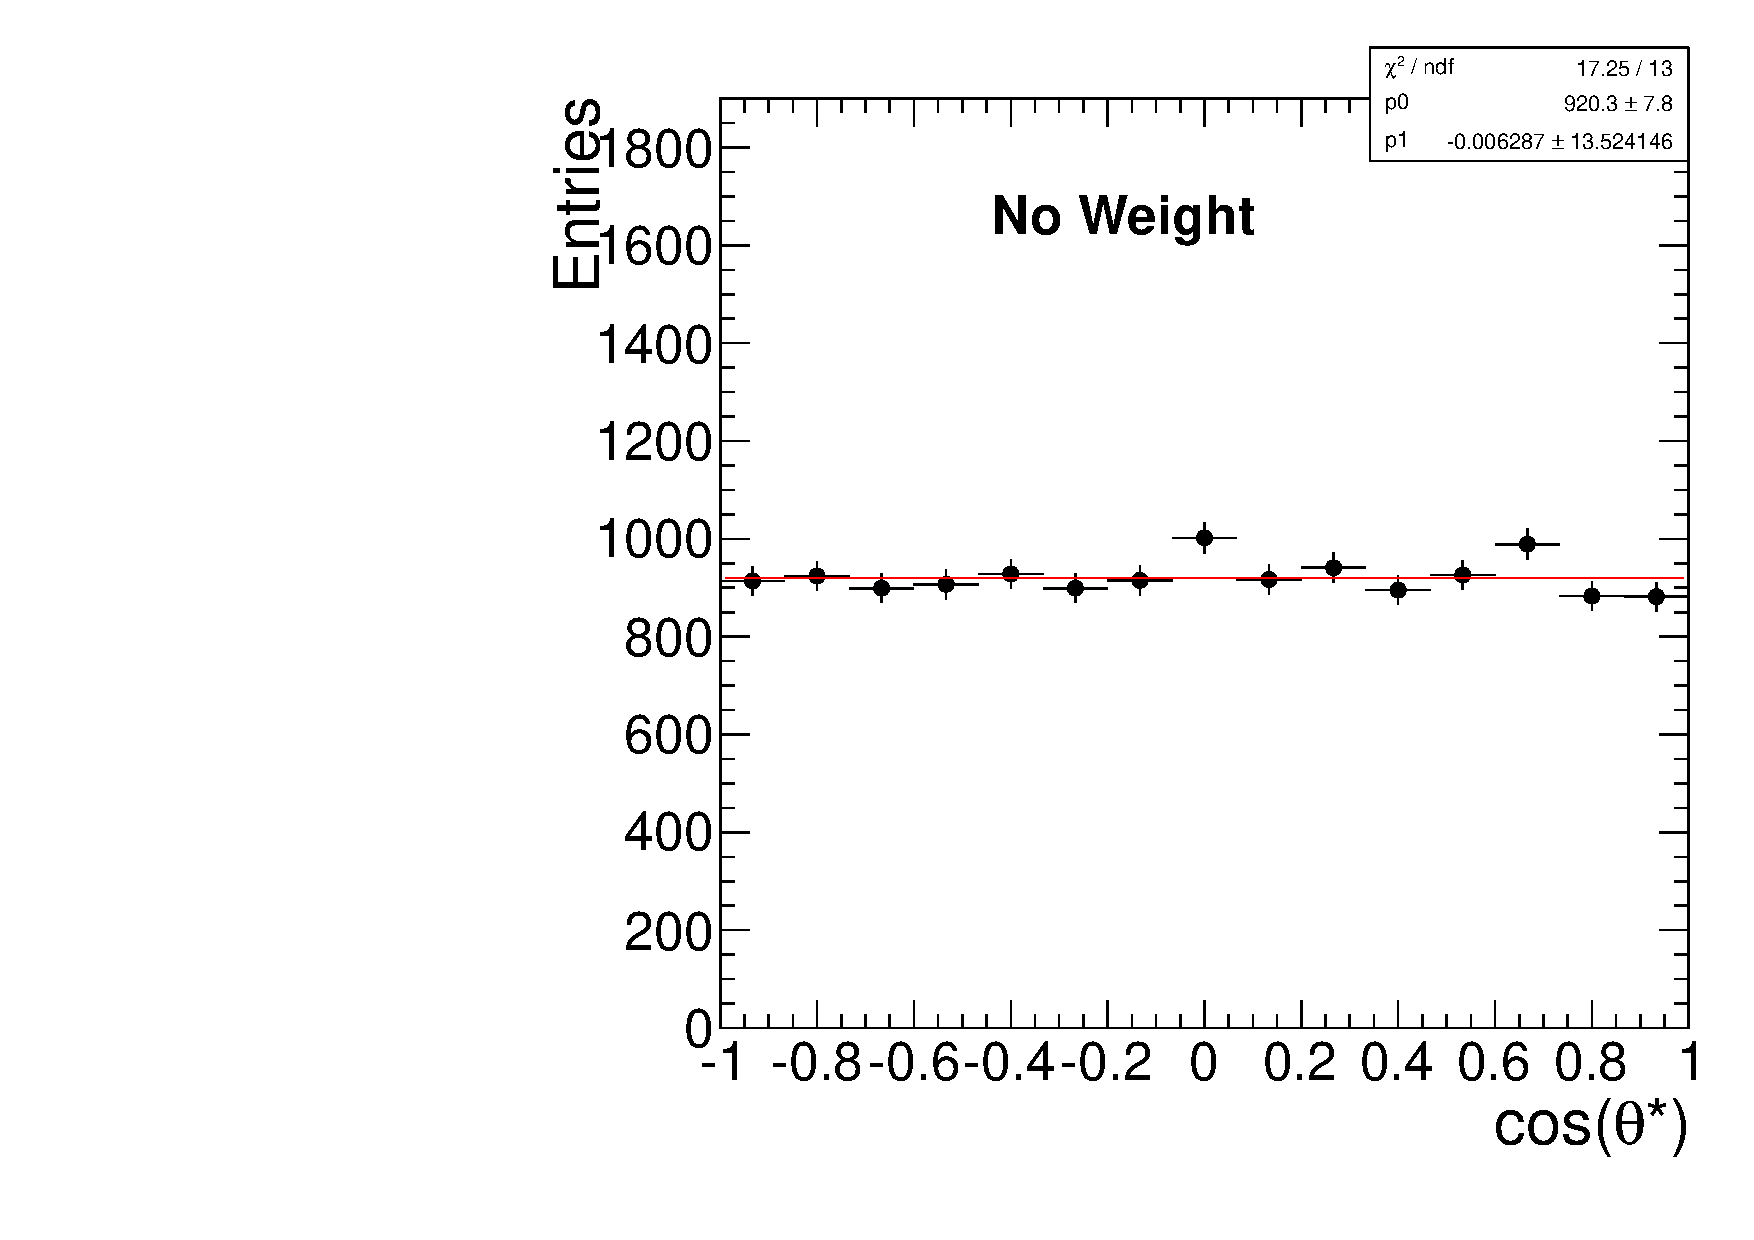
\includegraphics[width=0.325\linewidth]{plots/costheta.pdf}
	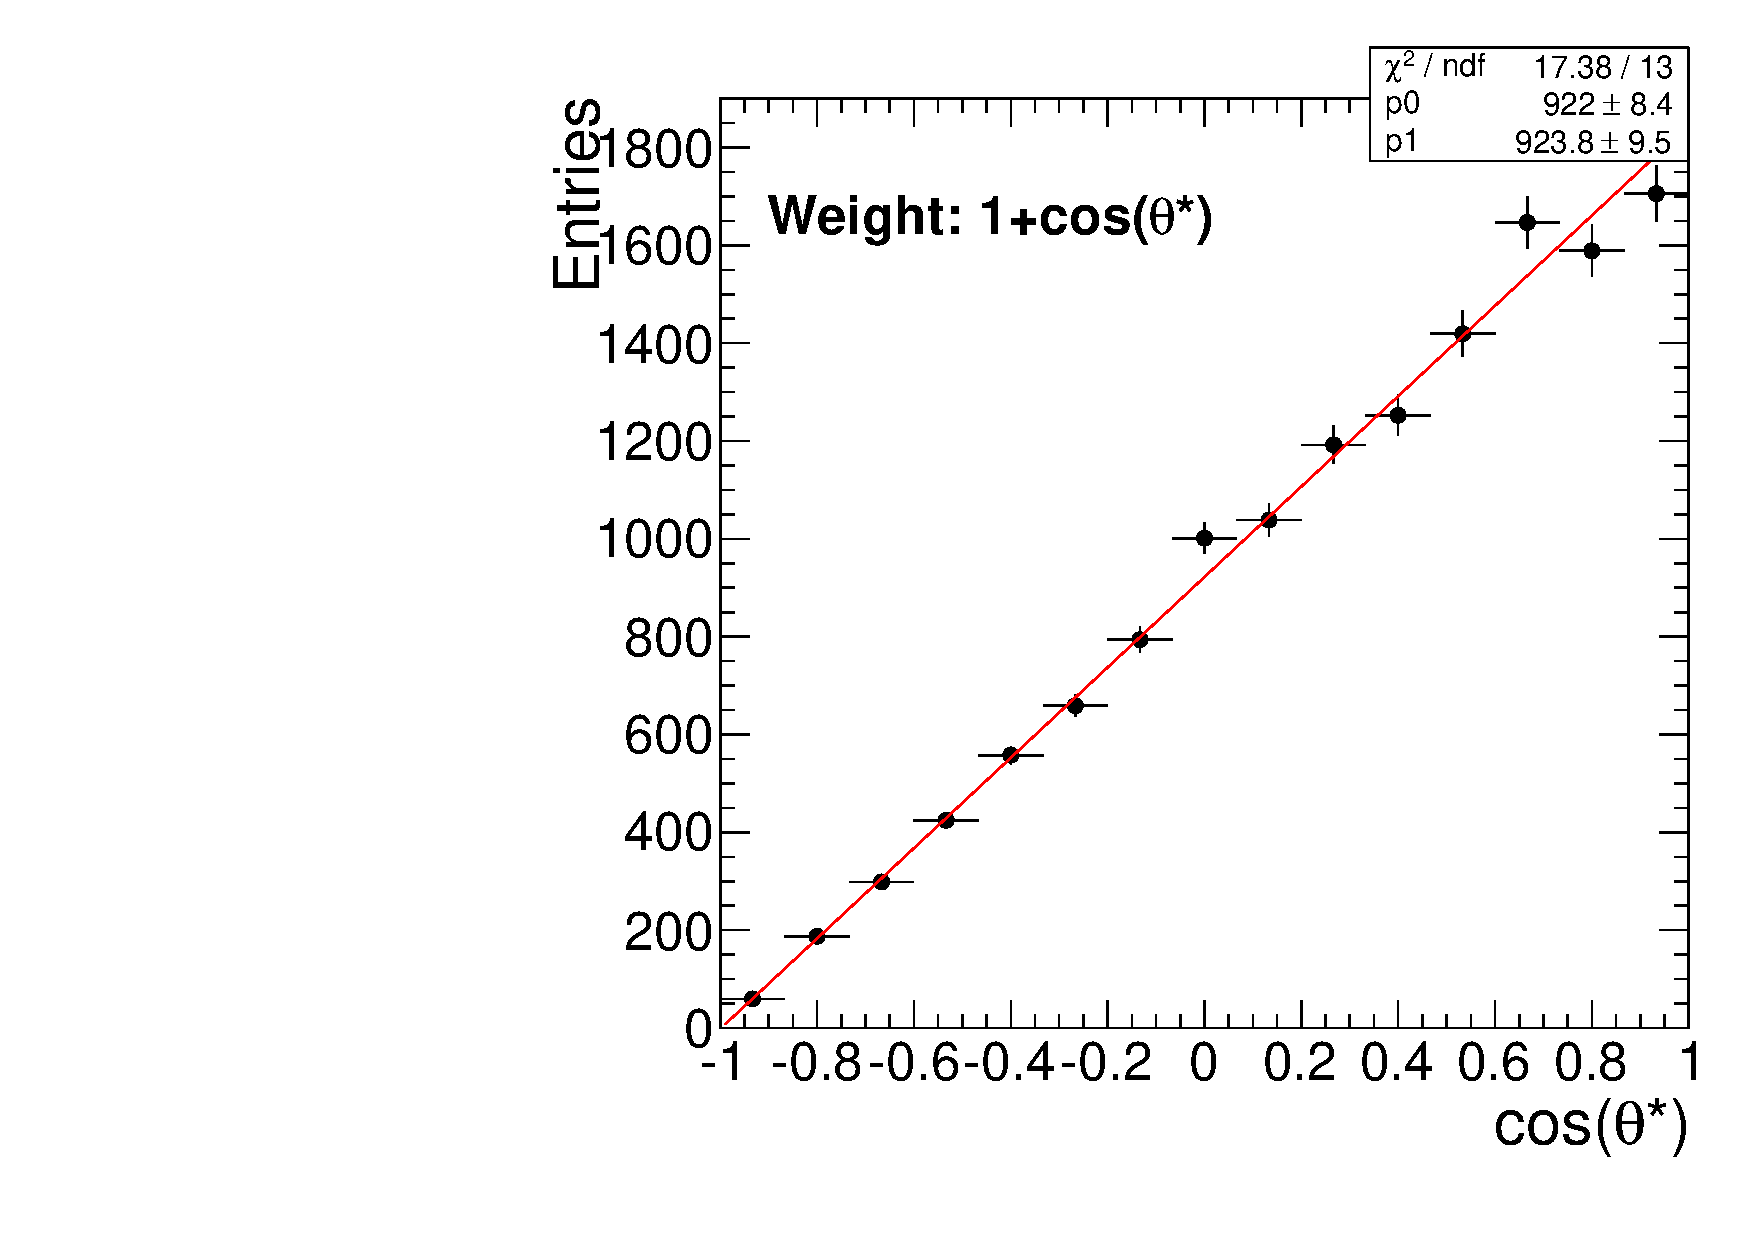
\includegraphics[width=0.325\linewidth]{plots/costheta_1p.pdf}
	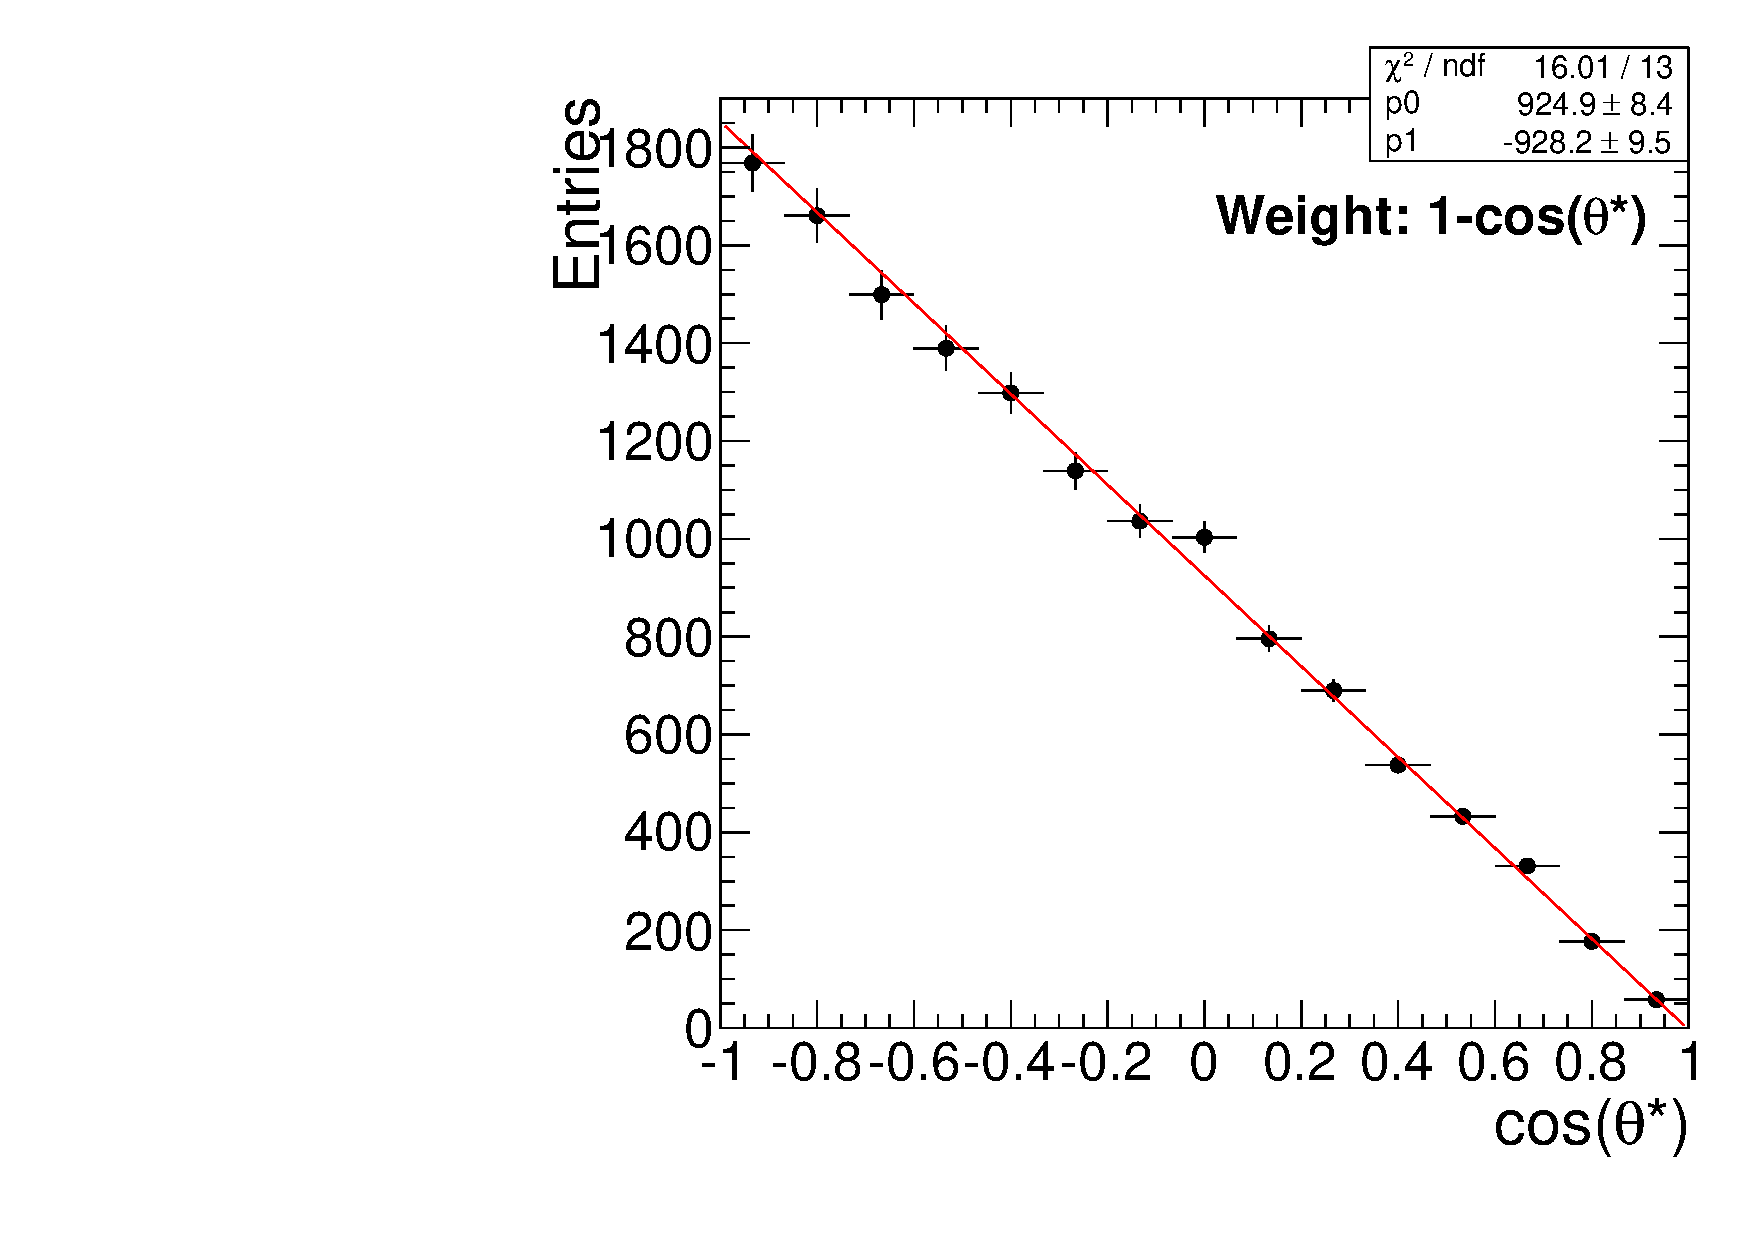
\includegraphics[width=0.325\linewidth]{plots/costheta_1m.pdf}
	\caption{
	  \label{fig:cosThetaStar}\protect 
          The default and reweighted $\cos\theta^{*}$ distributions. The $1 \pm \cos\theta^{*}$ weightings correspond to top polarizations of $\pm 1$.}
  \end{center}
\end{figure}

We find that reweighting to resemble a top polarization of +1 increases the signal acceptance by approximately 20-25\% relative to the default MC,
while using a top polarization of -1 decreases the signal acceptance by a similar amount. 